\documentclass{article}
\usepackage[utf8]{inputenc}

\title{Causal Decision Problems}
% \author{David Johnston}

\usepackage[mathscr]{euscript}
\usepackage{natbib}
\usepackage{graphicx}
\usepackage {tikz}
\usetikzlibrary {positioning}
\usepackage[a4paper, margin=0.7in]{geometry}
\setlength{\parskip}{1em}
\setlength{\parindent}{0em}
\usepackage{amsthm}
\usepackage{amsmath}
\usepackage{amssymb}
\usepackage{dsfont}
\usepackage{hyperref}
\usepackage{ stmaryrd }
\usepackage{csquotes}
\usepackage{wasysym}

\theoremstyle{definition}
\newtheorem{question}{Question}[section]
\newtheorem{definition}{Definition}[section]
\newtheorem{example}{Example}[section]
 
\theoremstyle{remark}
\newtheorem*{remark}{Remark}

 
\newtheorem{theorem}{Theorem}[section]
\newtheorem{corollary}{Corollary}[theorem]
\newtheorem{lemma}[theorem]{Lemma}
\newtheorem{corrolary}[theorem]{Corollary}

\setcounter{secnumdepth}{6}

\DeclareMathOperator*{\argmax}{arg\,max}
\DeclareMathOperator*{\argmin}{arg\,min}

\newcommand{\NC}[2]{\ensuremath{{#1}\not\to{#2}}}
\newcommand{\CI}{\mathrel{\text{\scalebox{1.07}{$\perp\mkern-10mu\perp$}}}}
\newcommand{\CII}{\mathrel{\text{\scalebox{1.07}{$\perp\mkern-10mu\perp\mkern-10mu\perp$}}}}
\newcommand{\GS}[1]{\ensuremath{\underline{\mathscr{#1}}}}
\newcommand{\PA}[2]{\ensuremath{\text{Pa}_{#1}(#2)}}
\newcommand{\ND}[2]{\ensuremath{\text{ND}_{#1}(#2)}}
\newcommand{\CH}[2]{\ensuremath{\text{Ch}_{#1}(#2)}}
\newcommand{\DE}[2]{\ensuremath{\text{De}_{#1}(#2)}}
\newcommand{\Insert}{\ensuremath{\text{insert}}}
\newcommand{\U}[1]{\ensuremath{\underline{#1}}}
\newcommand{\RV}[1]{\ensuremath{\mathsf{#1}}}
\newcommand{\XGA}[4]{\ensuremath{\RV{#2}^{\mathcal{#1}_{\overline{#3}}}_{#4}}}


\makeatletter
\newcommand*\bigcdot{\mathpalette\bigcdot@{.5}}
\newcommand*\bigcdot@[2]{\mathbin{\vcenter{\hbox{\scalebox{#2}{$\m@th#1\bullet$}}}}}
\makeatother

\newcommand\splitter[1]{%
\begin{tikzpicture}[scale=#1]
\draw (0,-1) -- (0,0);
\draw (0,0) to [bend right] (1,1);
\draw (0,0) to [bend left] (-1,1);

\end{tikzpicture}
}

\newcommand\stopper[1]{%
\begin{tikzpicture}[scale=#1]
\draw (0,-1) -- (0,0);
\node (E) at (0,0) {$\bigcdot$};

\end{tikzpicture}
}


\begin{document}

\maketitle

\tableofcontents
\newpage

\section{Notation}

\begin{itemize}
    \item Sets are capital letters $X,Q,A$
    \item Random variables are sans-serif $\RV{X,Q,A}$
    \item For a measurable set $X$, $\Delta(X)$ denotes the set of probability distributions over $X$.
    \item $\mathscr{P}(X)$ denotes the power set of $X$
    \item Given a probability space $(\Omega,\mathcal{F},\mu)$ and a random variable $\RV{X}$, $P_\mu(\RV{X})$ is the push-forward of $\mu$ by $\RV{X}$.
\end{itemize}

\section{Roadmap}

Written up, many areas need a bit of polish:

\begin{itemize}
    \item Definition of SCDP
    \begin{itemize}
        \item Consequences (with/without side information)
        \item Causal theories \& prospects
    \end{itemize}
    \item Reduction of SCDP to SDP 
    \begin{itemize}
        \item known consequence kernel
        \item identifiable/loss-identifiable
        \item Reverse: SDP to SCDP
    \end{itemize}
    \item Defining causal prospects:
    \begin{itemize}
        \item Trivial (skepticism/helplessness)
        \item From classes of CBNs
        \item Universal independence with/without trivial action
    \end{itemize}
\end{itemize}


Overall comment: a lot of work on fitting existing theories into SCDP framework. It would be nice to have examples or results that demonstrate why the SCDP framework is useful (i.e. ones that are difficult to pose or prove in other frameworks).

To do/could be done.
\begin{itemize}
    \item Why it is necessary for consequences to be a kernel rather than JPD
    \item Examples:
    \begin{itemize}
        \item Where a non-physical model is preferred (even with infinite samples? this is tough)
        \item Conservation laws (\emph{where was it I've seen these before})
    \end{itemize}
    \item Lattice structure of causal prospects
    \begin{itemize}
        \item Any interesting inclusion results for nested Markov models, invariance sets, ADMGs or potential outcomes/Causal Bayes Nets?
    \end{itemize}
    \item Weakening of CBNs:
    \begin{itemize}
        \item Any legitimate examples of invariance but not CMC?
        \item What is a partially complete causal invariance network?
        \item Which identifiability results from CBNs are relevant to CINs?
        \item Conservative PC and faithfulness without CMC
    \end{itemize}
    \item Approximate loss-identifiability
    \begin{itemize}
        \item Define (straightforward from loss-identifiability)
        \item Interesting examples of approximate identifiability
    \end{itemize}
    \item ``Very soft interventions'' (i.e. limited information about distribution of target variables)
    \item Sequential generalisation (vectorise everything?)
    \item Potential outcomes:
    \begin{itemize}
        \item Relating ignorability to universal independence
        \item ``Affine-transformed loss identifiability''
        \item When can counterfactual performance measures be posed as losses? (Is there are reduction from identifiable counterfactual questions to ordinary SDPs?)
    \end{itemize}
    \item ``Model complexity''
    \begin{itemize}
        \item Generalisation of independence of conditionals to causal prospects
        \item Axiomatic approach to complexity measures
        \item Vague idea that the ``same'' measure should apply to $\mu$ and $\mathscr{T}$ - clarify this
    \end{itemize}
    \item Meta-learning connection: when is $\mathscr{T}(\mu)$ an easily learnable class? (Also connection to Finn's work)
\end{itemize}

\include{Introduction}

\section{Markov Kernels and String Diagrams}



\begin{definition}[Markov kernel]
Given two measureable sets $(E,\mathcal{E})$ and $(F,\mathcal{F})$, a Markov kernel $K$ is a map $E\times \mathcal{F} \to [0,1]$ where
\begin{itemize}
    \item The map $x\mapsto K(B;x)$ is $\mathcal{E}$-measurable for every $B\in\mathcal{F}$
    \item The map $B\mapsto K(B;x)$ is a probability measure on $(F,\mathcal{F})$ for every $x\in E$ 
\end{itemize}

Writing the set of probability measures $(F,\mathcal{F})\to [0,1]$ as $\Delta(\mathcal{F})$, we can also write $K:E\to \Delta(\mathcal{F})$, to be read as ``$K$ maps from $E$ to probability measures on $(F,\mathcal{F})$''.

\end{definition}

\begin{definition}[Measure-kernel-function product]\label{def:kernel_products}
If $K$ is a Markov kernel from $(E,\mathcal{E})$ to $(F,\mathcal{F})$ and $\mu$ is a probability measure on $(E,\mathcal{E})$, then
\begin{align}
    \mu K(B)=\int_E \mu(dx) K(B;x),\qquad B\in\mathcal{F}
\end{align}
defines a probability measure $\mu K$ on $(F,\mathcal{F})$.

If $f$ is a nonnegative measurable function $F\to \mathbb{R}$ then
\begin{align}
    Kf(x) = \int_F K(dy;x)f(y), \qquad x\in E
\end{align}
is a nonnegative measureable function $E\to \mathbb{R}$.

If $L$ is a Markov kernel from $(F,\mathcal{F})$ to $(G,\mathcal{G})$, then
\begin{align}
    KL(B;x) = \int_F K(dy;x) L(B;y),\qquad x\in E, B\in \mathcal{G}
\end{align}
is a Markov kernel from $(E,\mathcal{E})$ to $(G,\mathcal{G})$. \cite{cinlar_probability_2011}
\end{definition}

\begin{definition}[Kernel Tensor product]
Given two kernels $K$ from $(E,\mathcal{E})$ to $(F,\mathcal{F})$ and $L$ from $(G,\mathcal{G})$ to $(H,\mathcal{H})$, the kernel $K\otimes L: (E\times G,\mathcal{F}\otimes \mathcal{H})\to [0,1]$ is defined:
\begin{align}
    K\otimes L([A,B];[x,y]) = K(A;x)L(B;y)
\end{align}
\end{definition}

\begin{lemma}[Countably generated $\pi$-systems]\label{lem:cgpisys}
Given a measurable space $(F,\mathcal{F})$ with countable $\mathcal{G}$ such that $\mathcal{F}=\sigma(\mathcal{G})$, then there is a countable $\pi$-system $\mathcal{H}$ such that $\mathcal{F}=\sigma(\mathcal{H})$.
\end{lemma}

\begin{proof}
Define $\mathcal{G}_0 = \mathcal{G}$ and $\mathcal{G}_{n+1} = \{A\cap B|A,B\in \mathcal{G}_n\}$. $\mathcal{G}_0$ is countable and $\mathcal{G}_n$ countable implies $\mathcal{G}_{n+1}$ is countable, so $\mathcal{G}_n$ is countable for all $n$.

Consider $\mathcal{G}_\infty = \bigcup_{n\in\mathbb{N}} \mathcal{G}_n$. $\mathcal{G}_\infty$ is closed under intersection; for any $A,B\in\mathcal{G}_\infty$, there is some $N\in \mathbb{N}$ such that $A,B\in \mathcal{G}_N$. Then $A\cap B\in\mathcal{G}_{N+1}$ so $A\cap B\in \mathcal{G}_\infty$. $\mathcal{G}_\infty$ is a countable union of countable sets, so it is a countable $\pi$-system.
\end{proof}

String diagrams are a helpful way to define more complex kernel products\cite{fong_causal_2013}. For any measurable space $(F,\mathcal{F})$, define the kernel
\begin{align}
    \splitter{0.2}:F\to \Delta(\mathcal{F}\otimes\mathcal{F})
\end{align} 
by 
\begin{align}
    \splitter{0.2}:(x,A)\mapsto \begin{cases}1 & (x,x)\in A\\ 0 & (x,x)\not\in A \end{cases}
\end{align} 
and given the indiscrete space $(*,\{\emptyset, *\})$ define
\begin{align}
    \stopper{0.2}:&F\to \Delta(\{\emptyset,*\});\\
                  &(x,*)\mapsto 1\\
                  &(x,\emptyset)\mapsto 0
\end{align}

and finally define
\begin{align}
    I_F:&F\times \mathcal{F} \to [0,1]\\
      &(x,A)\mapsto \delta_x(A)
\end{align}

Note that for any measure $\mu\in \Delta(\mathcal{F})$, $\mu I_F=\mu$, for any kernel $L:F\times \mathcal{G}\to [0,1]$ $IL=L$ and any kernel $M:E\to \mathcal{F}$, $MI=M$.

Given measurable spaces $(E,\mathcal{F})$, $(F,\mathcal{F})$ and $(G,\mathcal{G})$ and kernels $K_1:E\to \Delta(\mathcal{F})$, $K_2:E\to \Delta(\mathcal{G})$, $L:F\to \Delta(\mathcal{G})$ and $\splitter{0.2}:E\to \Delta(\mathcal{E}\otimes\mathcal{E})$, define

\begin{center}
    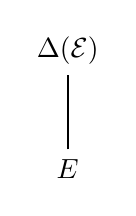
\begin{tikzpicture}[auto ,node distance =1 cm and 2cm ,on grid ,
    semithick ,
    variable/.style ={ circle ,top color =white , 
    draw , text=blue , minimum width =1 cm},
    kernel/.style={rectangle,draw}
    ]

\node (M) at (0,-1)  {$E$};
\node (N) at (0,0.5) {$\Delta(\mathcal{E})$};
\draw (M) --  (N);
\end{tikzpicture}
\end{center}

To be the kernel $I_E$, 

\begin{center}
    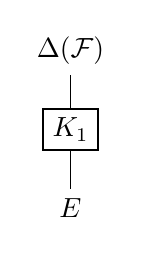
\begin{tikzpicture}[auto ,node distance =1 cm and 2cm ,on grid ,
    semithick ,
    variable/.style ={ circle ,top color =white , 
    draw , text=blue , minimum width =1 cm},
    kernel/.style={rectangle,draw}
    ]

\node (M) at (0,-1)  {$E$};
\node[kernel] (K) at (0,0) {$K_1$};
\node (N) at (0,1) {$\Delta(\mathcal{F})$};
\draw (M) -- (K);
\draw (K) -- (N);
\end{tikzpicture}
\end{center}

To be the kernel $K$. We write the kernel product $K_1L$ as

\begin{center}
    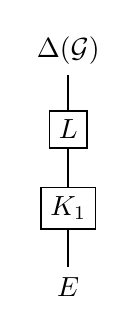
\begin{tikzpicture}[auto ,node distance =1 cm and 2cm ,on grid ,
    semithick ,
    variable/.style ={ circle ,top color =white , 
    draw , text=blue , minimum width =1 cm},
    kernel/.style={rectangle,draw}
    ]

\node (M) at (0,-1)  {$E$};
\node[kernel] (K) at (0,0) {$K_1$};
\node[kernel] (L) at (0,1) {$L$};
\node (N) at (0,2) {$\Delta(\mathcal{G})$};
\draw (M) -- (K);
\draw (K) -- (L);
\draw (L) -- (N);
\end{tikzpicture}
\end{center}

We understand the following two diagrams to refer to the product $\splitter{0.15}(K_1\otimes K_2)$

\begin{center}
    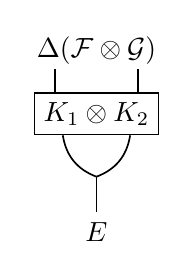
\begin{tikzpicture}[auto ,node distance =0.8 cm and 1cm ,on grid ,
    semithick ,
    variable/.style ={ circle ,top color =white , 
    draw , text=blue , minimum width =1 cm},
    kernel/.style={rectangle,draw}
    ]
    
    \node (M) at (0,-1)  {$E$};
    \node[kernel] (K1K2) at (0,0.5) {$K_1\otimes K_2$}; 
    \node (kleft) [left = 0.3cm of K1K2.south] {};
    \node (kright) [right = 0.3cm of K1K2.south] {};
    \node (klefttop) [left = 0.4cm of K1K2.north] {};
    \node (krighttop) [right = 0.4cm of K1K2.north] {};
    \node (N) [above = of K1K2] {$\Delta(\mathcal{F}\otimes\mathcal{G})$};
    \draw (M) -- (0,-0.3);
    \draw (0,-0.3) to [bend left] (kleft.center);
    \draw (0,-0.3) to [bend right] (kright.center);
    \draw (klefttop.center) to ++(0,0.3);
    \draw (krighttop.center) to ++(0,0.3);
    \end{tikzpicture}
    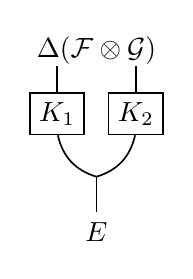
\begin{tikzpicture}[auto ,node distance =1 cm and 1cm ,on grid ,
    semithick ,
    variable/.style ={ circle ,top color =white , 
    draw , text=blue , minimum width =1 cm},
    kernel/.style={rectangle,draw}
    ]
    \node (M) at (0,-1)  {$E$};
    \node[kernel] (K1) at (-0.5,0.5) {$K_1$};
    \node[kernel] (K2) [right = of K1] {$K_2$};
    \node (C) [below right = 0.8cm and 0.5cm of K1] {};
    \node (N) [above right = 0.8cm and 0.5cm of K1] {$\Delta(\mathcal{F}\otimes\mathcal{G})$};
    \draw (M) to (C.center);
    \draw (C.center) to [bend right] (K2);
    \draw (C.center) to [bend left] (K1);
    \draw (K1) to ++(0,0.6);
    \draw (K2) to ++(0,0.6);
    \end{tikzpicture}
\end{center}

Of particular interest is the kernel $\splitter{0.15}(K_1\otimes I_E)$:
\begin{center}
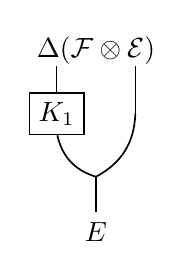
\begin{tikzpicture}[auto ,node distance =1 cm and 1cm ,on grid ,
semithick ,
variable/.style ={ circle ,top color =white , 
draw , text=blue , minimum width =1 cm},
kernel/.style={rectangle,draw}
]
    \node (M) at (0,-1)  {$E$};
    \node[kernel] (K1) at (-0.5,0.5) {$K_1$};
    \node (K2) [right = of K1] {};
    \node (C) [below right = 0.8cm and 0.5cm of K1] {};
    \node (N) [above right = 0.8cm and 0.5cm of K1] {$\Delta(\mathcal{F}\otimes\mathcal{E})$};
    \draw (M) to (C.center);
    \draw (C.center) to [bend right] (K2.center);
    \draw (C.center) to [bend left] (K1);
    \draw (K1) to ++(0,0.6);
    \draw (K2.center) to ++(0,0.6);
    \end{tikzpicture}
\end{center}

For any kernel $K:E\to\Delta(\mathcal{F})$, define $\overline{K}:=\splitter{0.15}(K_1\otimes I_E)$.

For any $\mu\in \Delta(\mathcal{E})$, we have $\mu \overline{K}(A\times B)=\int_B K(A;x) \mu(dx)$. If $(E,\mathcal{E})$ is a discrete space then we have $\mu \overline{K}(A\times B)=\sum_{x\in B} K_1(A;x) \mu(x)$\cite{fong_causal_2013}.

It is useful to define notions analogous to independence and conditional independence of random variables with respect to the kernel $K$. This is motivated by the notion of extended conditional independence:

\begin{definition}[Extended conditional independence (Dawid (2010)\cite{dawid_beware_2010})]\label{def:eci}
Given a measurable space $(F,\mathcal{F})$, a collection of parameters $S$ along with a variable $Y$ taking values in $S$, a set of $S$-indexed probability distributions $\{P_i\}_{i\in \mathcal{S}}\subset\Delta(\mathcal{F})$ and random variables $\RV{X}$, $\RV{V}$ on $(X,\mathcal{X})$ and $(V,\mathcal{V})$, extended conditional independence overloads the $\CI$ symbol to say
\begin{align}
    \RV{X}\CI_{\{P_i\}} Y | \RV{V}
\end{align}

Iff $P_i(\RV{X}|\RV{V})=P_j(\RV{X}|\RV{V})$ for all $i,j\in S$ wherever both $P_i(\RV{X}|\RV{V})$ and $P_j(\RV{X}|\RV{V})$ are defined.
\end{definition}

This motivates the following definitions of independence for a Markov kernel $K$:

\begin{definition}[Universal independence]\label{def:univ_indep}
Given measurable spaces $(E,\mathcal{E})$ and $(F,\mathcal{F})$, a kernel $K:E\times\mathcal{F}\to[0,1]$ and random variables $\RV{X}:(E,\mathcal{E})\to (X,\mathcal{X})$,$\RV{Y}:(F,\mathcal{F})\to (Y,\mathcal{Y})$, we say that $\RV{X}$ and $\RV{Y}$ are universally independent with respect to $K$ iff for all $\mu\in \Delta(\mathcal{E})$, $\RV{X}\CI_{\mu \overline{K}} \RV{Y}$. 

We will write this $\RV{Y} \CII_K \RV{X}$.

Given a third random variable $\RV{V}:( F,\mathcal{F})\to(V,\mathcal{V})$, $\RV{X}$ and $\RV{Y}$ are universally conditionally independent with respect to $K$ and $\RV{V}$ iff for all $\mu\in \Delta(\mathcal{E})$, $\RV{X}\CI_{\mu \overline{K}} \RV{Y}|\RV{V}$.

We will write this $\RV{Y} \CII_K \RV{X} | \RV{V}$.
\end{definition}

\begin{definition}[Domain invariance]\label{def:domain_indep}
Given measurable spaces $(E,\mathcal{E})$ and $(F,\mathcal{F})$, a kernel $K:E\times\mathcal{F}\to[0,1]$ and a random variable $\RV{Y}:( F,\mathcal{F})\to (Y,\mathcal{Y})$, we say $\RV{Y}$ is domain invariant with respect to $K$ if, defining $P_{K(\cdot;e)}(\RV{Y}):=Y_*K(\cdot;e)$, we have $P_{K(\cdot;e)}(\RV{Y}) = P_{K(\cdot;e')}(\RV{Y})$ for all $e,e'\in E$.

Given $\RV{V}:(F,\mathcal{F})\to (V,\mathcal{V})$, $\RV{Y}$ is domain invariant with respect to $K$ conditional on $\RV{V}$ if $P_{K(\cdot;e)}(\RV{Y}|\RV{V}) = P_{K(\cdot;e')}(\RV{Y}|\RV{V})$ for all $e,e'\in E$ wherever both sides are uniquely defined.
\end{definition}

Domain conditional invariance is clearly closely connected with extended conditional independence. In particular, given $\{P_i\}_{i\in \mathcal{S}}$ we can define the kernel $K_S:i\mapsto P_i$ in which case extended conditional independence is equivalent to domain conditional invariance with respect to $K_S$.

In addition, universal independence is equivalent to domain independence under weak conditions.

\begin{theorem}[Equivalence of universal and domain independence]
Given measurable spaces $(E,\mathcal{E})$, $(F,\mathcal{F})$ along with random variables $\RV{X}:(E,\mathcal{E})\to (X,\mathcal{X})$, $\RV{Y}:(F,\mathcal{F})\to (Y,\mathcal{Y})$ and a kernel $K:(E,\mathcal{F})\to [0,1]$, the following statements are equivalent:
\begin{enumerate}
    \item $\RV{X}\CII_K \RV{Y}$
    \item $\RV{Y}$ is domain independent with respect to $K$ 
\end{enumerate}

\end{theorem}

\begin{proof}
If either $\RV{X}$ or $\RV{Y}$ are constant functions, 1 and 2 hold trivially. Suppose for the following that they are not constant.

$1\implies 2$:
Suppose the converse. Then we have some $u,u'\in E$ such that $P_{K(\cdot;u)}(\RV{Y})\neq P_{K(\cdot;u')}(\RV{Y})$. There is some $C\in \mathcal{Y}$  such that $K(\RV{Y}^{-1}(C);u)\neq K(\RV{Y}^{-1}(C);u')$. Let $A^C_u=\{x|K(\RV{Y}^{-1}(C);x)=K(\RV{Y}^{-1}(C);u)\}$. We know $A_u, A_{u'}\in \mathcal{E}$ and $A_u$ and $A_{u'}$ are non-empty and disjoint.

We also have some $v\in E$ such that $B_v=\RV{X}^{-1}(\RV{X}(v))$ and $B_v^C$ are both nonempty.

\textbf{Case 1:} $B_v\cap A_u\neq \emptyset$ and $B_v^C \cap A_{u'}\neq \emptyset$. Let $\delta_1=\delta_{(B_v\cap A_u)\cup(B_v^C \cap A_{u'})}$. Then we have
\begin{align}
    P_{\delta_1\overline{K}}(\RV{Y}\in C|\RV{X}\in B_v) &= P_{K(\cdot;u)}(\RV{Y}\in C)\\
    &\neq P_{K(\cdot;u')}(\RV{Y}\in C)\\
    &=  P_{\delta_1\overline{K}}(\RV{Y}\in C|\RV{X}\in B^C_v)
\end{align}
This contradicts the assumption that $\RV{X}\CI_{\mu\overline{K}} \RV{Y}$ for all $\mu\in\Delta(\mathcal{F})$.

\textbf{Case 2:} $B_v\cap A_{u'}\neq \emptyset$ and $B_v^C \cap A_{u}\neq \emptyset$. This is analogous to case 1 with symbols interchanged.

\textbf{Case 3:} $B_v\cap A_u\neq \emptyset$ and $B_v \cap A_{u'}\neq \emptyset$. Consider an arbitrary $u''\in B_v^C$. We have $P_{K(\cdot;u)}(\RV{Y})\neq P_{K(\cdot;u'')}(\RV{Y})$ or $P_{K(\cdot;u')}(\RV{Y})\neq P_{K(\cdot;u'')}(\RV{Y})$. By assumption $B_v^C\cap A_{u''}\neq \emptyset$. Then an analogous argument to case 1 indicates that $\RV{X}$ and $\RV{Y}$ are not universally independent in this case.

\textbf{Case 4:} $B^C_v\cap A_u\neq \emptyset$ and $B^C_v \cap A_{u'}\neq \emptyset$. This is analogous to case 3 with symbols interchanged.

$2\implies 1$:
We have for all $u\in E$, $P_{K(\cdot;u)}(\RV{Y})=P_K(\RV{Y})$ for some $P_K\in \Delta(\mathcal{Y})$. But $P_{K(\cdot;u)}(\RV{Y}\in A) = K(\RV{Y}^{-1}(A);u)$ and $P_{\mu\overline{K}}(\RV{X}\in B,\RV{Y}\in A) = \int_{\RV{X}^{-1}(B)} K(\RV{Y}^{-1}(A);u) \mu(du)=P_K(\RV{Y}\in A)\mu(\RV{X}^{-1}(B))$.

\end{proof}

\begin{theorem}[Equivalence of universal and domain conditional independence]\label{th:univ_dom_cond_equiv}
Given measurable spaces $(E,\mathcal{E})$, $(F,\mathcal{F})$ along with random variables $\RV{X}:(E,\mathcal{E})\to (X,\mathcal{X})$, $\RV{Y},\RV{V}:(F,\mathcal{F})\to (Y,\mathcal{Y})$ and a kernel $K:(E,\mathcal{F})\to [0,1]$, if $\RV{Y}\otimes \RV{V}$ is countably generated then the following statements are equivalent:
\begin{enumerate}
    \item $\RV{X}\CII_K\RV{Y}|\RV{V}$
    \item $\RV{Y}$ is domain independent with respect to $K$ conditional on $\RV{V}$.
\end{enumerate}

\end{theorem}

\begin{proof}
If either $\RV{X}$ or $\RV{Y}$ are constant functions, 1 and 2 hold trivially. Suppose for the following that they are not constant.


$1\implies 2$:
Suppose the converse. Then we have some $u,u'\in E$ such that
\begin{align}
    P_{K(\cdot;u)}(\RV{Y}|\RV{V})\neq P_{K(\cdot;u')}(\RV{Y}|\RV{V})\label{eq:cond_ieq}
\end{align} 
where both quantities are uniquely defined. Let $\mathcal{Z}$ be a countable $\pi$-system generating $\mathcal{Y}\otimes \mathcal{V}$ (Lemma \ref{lem:cgpisys}). Because $(\RV{Y}\times\RV{V})_*K(\cdot;u)$ is a finite measure on $\mathcal{Y}\otimes \mathcal{V}$ for all $u\in E$, equality of $(\RV{Y}\times\RV{V})_*K(\cdot;u)$ and $(\RV{Y}\times\RV{V})_*K(\cdot;u')$ on $\mathcal{Z}$ is sufficient to show that 
\begin{align}
    (\RV{Y}\times\RV{V})_*K(\cdot;u)=(\RV{Y}\times\RV{V})_*K(\cdot;u')\label{eq:joint_eq}
\end{align} 
However, if Eq. \ref{eq:joint_eq} holds then Eq. \ref{eq:cond_ieq} cannot.

Therefore there must be some $C\in \mathcal{Z}$ such that 
\begin{align}
    K((\RV{Y}\times \RV{V})^{-1}(C);u)\neq K((\RV{Y}\times \RV{V})^{-1}(C);u')\label{eq:pointwise_joint_ieq}
\end{align}

For some $C\in\mathcal{Z}$, let $A^{C}_u=\{x|K((\RV{Y}\times\RV{V})^{-1}(C);x)=K((\RV{Y}\times\RV{V})^{-1}(C);u)\}$. Further, let $A_u=\bigcap_{C\in\mathcal{Z}} A^{C}_u$. Because $\mathcal{Z}$ is countable, we know $A_u, A_{u'}\in \mathcal{E}$ and by Eq. \ref{eq:pointwise_joint_ieq} $A_u$ and $A_{u'}$ are disjoint and non-empty.

We also have some $v\in E$ such that $B_v=\RV{X}^{-1}(\RV{X}(v))$ and $B_v^C$ are both nonempty.

\textbf{Case 1:} $B_v\cap A_u\neq \emptyset$ and $B_v^C \cap A_{u'}\neq \emptyset$. Let $\delta_1=\delta_{(B_v\cap A_u)\cup(B_v^C \cap A_{u'})}$. Note that
\begin{align}
    P_{\delta_1\overline{K}}(\RV{Y}\in C,\RV{V}\in D|\RV{X}\in B_v) &= P_{K(\cdot;u)}(\RV{Y}\in C,\RV{V}\in D)\\
\end{align}
for all $C\in \mathcal{Y}$ and $D\in \mathcal{V}$. 

Therefore, wherever the following conditional probabilities are uniquely defined by the joint probability of $\RV{Y}$ and $\RV{V}$, we have
\begin{align}
    P_{\delta_1\overline{K}}(\RV{Y}|\RV{V},\RV{X}\in B_v) &= P_{K(\cdot;u)}(\RV{Y}|\RV{V})\\
\end{align}
and similarly for $\RV{X}\in B_v^C$. But we have some $C\in \mathcal{Y}$, $D\in \mathcal{V}$ such that $P_{K(\cdot;u)}(\RV{Y}\in C|\RV{V}\in D)$ and $P_{K(\cdot;u')}(\RV{Y}\in C|\RV{V}\in D)$ are uniquely defined for their respective joint distributions and
\begin{align}
    P_{K(\cdot;u)}(\RV{Y}\in C|\RV{V}\in D)&\neq P_{K(\cdot;u')}(\RV{Y}\in C|\RV{V}\in D)\\
    \implies P_{\delta_1\overline{K}}(\RV{Y}|\RV{V},\RV{X}\in B_v) &\neq  P_{\delta_1\overline{K}}(\RV{Y}|\RV{V},\RV{X}\in B^C_v)
\end{align}
This contradicts the assumption that $\RV{X}\CI_{\mu\overline{K}} \RV{Y}|\RV{V}$ for all $\mu\in\Delta(\mathcal{F})$.

\textbf{Case 2:} $B_v\cap A_{u'}\neq \emptyset$ and $B_v^C \cap A_{u}\neq \emptyset$. This is analogous to case 1 with symbols interchanged.

\textbf{Case 3:} $B_v\cap A_u\neq \emptyset$ and $B_v \cap A_{u'}\neq \emptyset$. Consider an arbitrary $u''\in B_v^C$. We have $P_{K(\cdot;u)}(\RV{Y}|\RV{V})\neq P_{K(\cdot;u'')}(\RV{Y}|\RV{V})$ or $P_{K(\cdot;u')}(\RV{Y}|\RV{V})\neq P_{K(\cdot;u'')}(\RV{Y}|\RV{V})$. By assumption $B_v^C\cap A_{u''}\neq \emptyset$. Then an analogous argument to case 1 indicates that $\RV{X}$ and $\RV{Y}$ are not universally independent in this case.

\textbf{Case 4:} $B^C_v\cap A_u\neq \emptyset$ and $B^C_v \cap A_{u'}\neq \emptyset$. This is analogous to case 3 with symbols interchanged.

$2\implies 1$:
We have for all $u\in E$, $P_{K(\cdot;u)}(\RV{Y}|\RV{V})=P_K(\RV{Y}|\RV{V})$ for some $P_K\in \Delta(\mathcal{Y})^{\mathcal{V}}$...

\end{proof}

We will simply refer to universal independence, and use the symbol $\CII_K$ to express both notions, with the caveat that unless we can lift \ref{th:univ_dom_cond_equiv} to countably generated spaces the equivalence has not been shown to hold for continuous variables $\RV{Y}$ or $\RV{V}$ and even if we can then there may be pathological cases where the spaces are not standard Borel spaces.

\textbf{Conjecture:} The relationship between mutual information and conditional independence is analogous to the relationship between channel capacity and universal conditional independence.
\section{Causal Decision Problems}

A causal decision problem extends a statistical decision problem in that, while an SDP provides us with a loss $D\times \Delta(\mathcal{F})\to [0,\infty)$ that evaluates (decision, state) pairs, a CDP gives us a loss from $\Delta(\mathcal{F})\to [0,\infty)$ that evaluates only consequences. Evaluating the quality of a decsion in an CDP therefore requires an object of the type $D\to \Delta(\mathcal{F})$, which we call a \emph{consequence kernel}.

\begin{definition}[Consequence kernel]
Given a measurable space $(\Omega,\mathcal{F})$ and a measurable decision set $(D,\mathcal{D})$, a consequence kernel is a Markov kernel $\kappa:D \to \Delta(\mathcal{F})$.
\end{definition}

\begin{definition}[Causal Decision Problem]
A causal decision problem (CDP) is a tuple $\langle (\Omega,\mathcal{F},\kappa^*), (D,\mathcal{D}), L, \mathbf{K} \rangle$. The triple $(\Omega,\mathcal{F},\kappa^*)$ is given by the environment, where $\Omega$ is the sample space and $\mathcal{F}$ is a $\sigma$-algebra on $\Omega$. We posit that a true consequence kernel $\kappa^*$ exists which is only known to belong to the class $\mathbf{K}\subset \Delta(\mathcal{F})^D$.

The measurable set $D$ represents the decisions available, and $L:\Delta(\mathcal{F})\to [0,\infty)$ is the loss.

The objective of a causal decision problem is to choose a stochastic decision $\phi\in \Delta(\mathcal{D})$ minimising the loss.
\end{definition}

In a causal decision problem, the class $\mathbf{K}$ represents the given background knowledge about how the world works. A generalised statistical causal decision problem is a causal decision problem in which, rather than a consequence class $\mathbf{K}$, we are given a random variable and a \emph{generalised causal prospect}.

\begin{definition}[Generalised Causal Theory]\label{def:gen_causal_theory}
Given a measurable space $(\Omega,\mathcal{F})$, a random variable $\RV{X}:\Omega\to X$ and a decision set $D$, a causal theory is a map $\tau:X \to \Delta(\mathcal{F})^D$ where $\Delta_{\tau}(\mathcal{F})\subset \Delta(\mathcal{F})$ is the domain of $\tau$. A causal theory maps a measurable set to a consequence kernel.

Given a set of probability distributions $\mathbf{P}\subset \Delta(\mathcal{F})$ a causal theory $\tau$ induces a map $\underline{\tau}:2^{\Delta(\mathcal{F})}\to 2^{D\times \Omega \to \Delta(\mathcal{F})}$ defined by $\underline{\tau}:\mathbf{P}\mapsto \{\tau(P)|P\in\mathbf{P}\cap \Delta_{\tau}(\mathcal{F})\}$. We overload the definition of a causal theory to say a causal theory also maps sets of distributions to sets of consequences.

A pair $\mathbf{P}\subset \Delta(\mathcal{F}), \tau$ is \emph{invalid} if $\underline{\tau}(\mathbf{P})=\emptyset$.

Given a set of probability distributions $\mathbf{P}\subset \Delta(\mathcal{F})$ a causal theory $\tau$ induces a map $\underline{\tau}:2^{\Delta(\mathcal{F})}\to 2^{D\times \Omega \to \Delta(\mathcal{F})}$ defined by $\underline{\tau}:\mathbf{P}\mapsto \{\tau(P)|P\in\mathbf{P}\cap \Delta_{\tau}(\mathcal{F})\}$. We overload the definition of a causal theory to say a causal theory also maps sets of distributions to sets of consequences.

\textbf{Example:} We can construct a causal theory from a directed acyclic graph. Suppose we have a DAG $\mathcal{G}$ with nodes $\RV{V}=\{\RV{V}_i|i\in U\}$ and associated measurable space $V=\prod_{i\in U} V_i$. Given $S\subset U$, define a bijection $f:D\to V_S$ such that $f:d_x\mapsto x$ for all $(d_x,x)\in D\times V_S$. Suppose we also have random variables $\RV{V}_i$ on $V_i$ for each $i\in U$ with joint distribution $P_\mu(\RV{V})$. Then $\mathcal{G}$ defines a causal theory $\tau_{\mathcal{G}}:d_x\mapsto P_{\mathcal{G}}(\RV{V}|do(X=x))$. If $V_S=V$ then $\mathcal{G}$ is a causal Bayesian network compatible with $\{\tau_{\mathcal{G}}(P_\mu)(x)|x\in V\}$.
\end{definition}

\begin{definition}[Causal prospect]\label{def:causal_prospect}
Given a measurable space $(\Omega,\mathcal{F})$ and a decision set $D$, a causal prospect $\mathscr{T}$ is a set of causal theories.

A causal prospect defines a map $\Delta(\mathcal{F})\to 2^{D\times \Omega \to \Delta(\mathcal{F})}$ by $\mathscr{T}:P\mapsto \{\tau(P)|\tau\in\mathscr{T}\wedge P\in \Delta_{\tau}(\mathcal{F})\}$ for $P\in \Delta(\mathcal{F})$. A causal prospect maps a probability distribution to a set of consequences.

Given some $\mu\in \Delta(\mathcal{F})$, we will define the range of $\mathscr{T}(\mu)$ to be the set $\{\nu\in \Delta(\mathcal{F})|\exists K\in \mathscr{T}(\mu)\wedge \exists d\in D:K(d)=\nu\}$. That is the range of $\mathscr{T}(\mu)$ is the set of every distribution on $\mathcal{F}$ that is considered ``possible'' by $\mathscr{T}$ given the distribution $\mu$.

Similarly, a causal prospect defines a map $\underline{\mathscr{T}}:2^{\Delta(\mathcal{F})}\to 2^{D\times \Omega\to \Delta(\mathcal{F})}$ by $\mathscr{T}:\mathbf{P}\mapsto \{\underline{\tau}(\mathbf{P})|\tau\in\mathscr{T}\}$ for $\mathbf{P}\subset \Delta(\mathcal{F})$. We overload the definition of causal prospect to say it also maps sets of probability distributions to sets of consequences.
\end{definition}
\begin{figure}[ht]
    \centering
    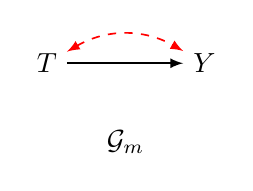
\begin{tikzpicture}[-latex ,auto ,node distance =1 cm and 2cm ,on grid ,
    semithick ,
    variable/.style ={ circle ,top color =white , 
    draw , text=blue , minimum width =1 cm},
    kernel/.style={rectangle,draw}
    ]
    \node (T1) {$T$};
    \node (Y1) [right = of T1] {$Y$};
    \node (G2) [below right = 1cm and 1cm of T1] {$\mathcal{G}_m$};
    \draw (T1) -- (Y1);
    \draw[latex-latex,dashed,red] (T1) [bend left] to (Y1);
    \end{tikzpicture}
    \caption{A marginal DAG indicating an unobserved common cause of $\RV{T}$ and $\RV{Y}$ defines a causal prospect.}
    \label{fig:theory_strength}
\end{figure}

\textbf{Example:} A causal prospect is defined by a marginal DAG $\mathcal{G}_m$ (figure \ref{fig:theory_strength}). A marginal DAG represents a marginal distribution over unobserved variables\cite{evans_graphs_2016}. Suppose we have measurable sets $T,Y=\{0,1\}$ with random variables $\RV{T},\RV{Y}$ distributed according to $P_\mu(\RV{T},\RV{Y})$, and the decision set $D=\{0,1\}$ also. Fix some measurable set $U$ and let $\mathbf{P}_U = \{P\in \Delta(T\times Y\times U)|P(\RV{T},\RV{Y})=P_\mu(\RV{T},\RV{Y})\}$. Then 
\begin{align}
    \mathscr{T}_{\mathcal{G}_m}:P_\mu(\RV{T},\RV{Y})\mapsto \{\kappa(\RV{T},\RV{Y}|d)|\exists P\in \mathbf{P}_U: \kappa(\RV{T},\RV{Y}|d)=\delta_d(\RV{T})\int_{U}P(\RV{Y}|\RV{T},\RV{U})dP(\RV{U})\} \label{eq:doct_hidden}
\end{align}


\begin{definition}[Statistical Causal Decision Problem]\label{def:SCDP}
A statistical causal decision problem (SCDP) is a tuple $\langle (\Omega,\mathcal{F},\mu,\kappa^*), D, \mathscr{T}, L\rangle$. $(\Omega,\mathcal{F},\mu)$ is a probability space and $\kappa$ is some ``true'' consequence kernel. $(D,\mathcal{D})$ is a measurable space. $\mathscr{T}$ is a causal prospect and $L$ is a loss $L:\Delta(\mathcal{F}\otimes\mathcal{D}\otimes\mathcal{F})\to [0,\infty)$.

The tuple $(\Omega,\mathcal{F},\mu,\kappa^*)$ are given by the environment and may not be directly observed.
\end{definition}


The \emph{aim} of a statistical causal decision problem requires some elaboration.

\begin{definition}[Realisable]
An SCDP $\langle (\Omega,\mathcal{F},\mu,\kappa^*), D, \mathscr{T}, L\rangle$ is realisable if $\kappa^*\in \mathscr{T}(\mu)$.
\end{definition}
% We will call any causal theory $\tau$ ``reliable'' if $\tau(\mu)=\kappa^*$. Note that there may be many different causal theories with this property.


\begin{definition}[Decision kernel]
Given a sample space $\Omega$ and a decision space $D$, a decision kernel is a stochastic map $\delta:\Omega \to \Delta(D)$.

We will usually define some random variable $\RV{Y}:\Omega\to Y$ and the decision kernel will be constant on $\RV{Y}^{-1}(y)$ for all $y\in Y$.
\end{definition}

\begin{definition}[Observation-decision-consequence joint distribution]
Given a statistical causal decision problem $\langle (\Omega,\mathcal{F},\mu), D, \mathscr{T},\kappa^*, L\rangle$ and a decision kernel $J:\Omega \to \Delta(D)$, we can define for some $K\in \mathscr{T}(\mu)$ the distribution $P^{J K}_\mu\in \Delta(\Omega \times D \times \Omega)$ by

\begin{center}
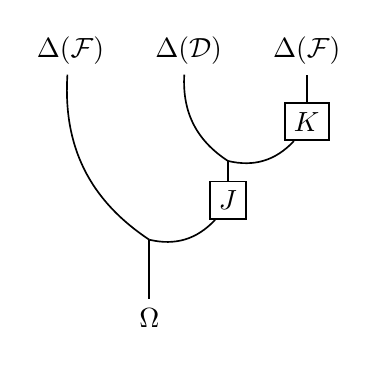
\begin{tikzpicture}[auto ,node distance =1 cm and 2cm ,on grid ,
    semithick ,
    variable/.style ={ circle ,top color =white , 
    draw , text=blue , minimum width =1 cm},
    kernel/.style={rectangle,draw}
    ]
\node (M) at (0,-1) {$\Omega$};
\node[kernel] (K) at (1,0.5) {$J$};
\node[kernel] (T) at (2,1.5) {$K$};
\node (DF) at (-1,2.4) {$\Delta(\mathcal{F})$};
\node (DD) at (0.5,2.4) {$\Delta(\mathcal{D})$};
\node (DF2) at (2,2.4) {$\Delta(\mathcal{F})$};
\draw (M) -- (0,0);
\draw (0,0) to [bend left] (DF);
\draw (0,0) to [bend right] (K);
\draw (K) to (1,1);
\draw (1,1) to [bend right] (T);
\draw (1,1) to [bend left] (DD);
\draw (T) to (DF2);
\end{tikzpicture}
\end{center}

We can also write, for $O\times E\times C\in \mathcal{F}\otimes \mathcal{D} \otimes\mathcal{F}$,

\begin{align}
    P^{J K}_\mu (O\times E\times C) = \int_O \int_E  K(C ;y,x^o) J(\mathrm{d}y; x^o) \mu(\mathrm{d}x^o)
\end{align}

Given some random variable $\RV{X}:\Omega\to X$, define random variables $\RV{X}^o,\RV{X}^c:\Omega\times D\times \Omega\to X$ by $\RV{X}^o:(\omega^o,d,\omega^c)\mapsto \RV{X}(\omega^o)$ and $\RV{X}^c:(\omega^o,d,\omega^c)\mapsto \RV{X}(\omega^c)$. Define $\RV{D}:(\omega^o,d,\omega^c)\mapsto d$. Then $P^{J K}_\mu(\RV{X}^o,\RV{D},\RV{X}^c)$ is the push forward of $P^{J K}_\mu$ by $\RV{X}^o\otimes\RV{D}\otimes\RV{X}^c$.



\end{definition}

We are now in a position to define the causal risk $R:\Delta(\mathcal{F})\times  \Delta(\mathcal{F})^{D\times \Omega} \times \Delta(D)^{\Omega}\to [0,\infty)$ by
\begin{align}
    R:(\nu,K,J)\mapsto L(P^{J K}_\nu) \label{eq:risk}
\end{align}

Define the objective risk of a decision kernel $J$ to be
\begin{align}
    R(\mu,\kappa^*,J) \label{eq:objective_risk}
\end{align}

The aim of a statistical causal decision problem is to find a decision kernel $J$ minimising the objective risk.

\subsection{Reduction to Ordinary Statistical Decision Problem}



\begin{definition}[Loss that depends only on consequences]
We will say a loss $L$ depends only on the consequences if, given any $\nu,\eta\in \Delta(\mathcal{F}\otimes\mathcal{D}\otimes\mathcal{F})$ and any $C\in \mathcal{F}$, we have
\begin{align}
    \nu(\Omega\times D\times C) &= \eta(\Omega\times D\times C) \\
    \implies L(\nu) &= L(\eta)
\end{align}
I anticipate that most losses will only depend on the consequences.
\end{definition}

\begin{definition}[Linear loss]
A loss $L$ is linear if, for $\nu,\eta\in \Delta(\mathcal{F}\otimes\mathcal{D}\otimes\mathcal{F})$, $L(\alpha\nu + (1-\alpha)\eta) = \alpha L(\nu) + (1-\alpha) L(\eta)$.
\end{definition}

\begin{theorem}[Reduction to ordinary statistical decision problem]\label{th:id_scdp}
Given an SCDP $\langle (\Omega,\mathcal{F},\mu,\kappa^*), D, \mathscr{T}, L\rangle$ where the true consequence kernel $\kappa^*$ is known and the loss $L$ is linear and depends only on the consequences, the problem can be reduced to an ordinary statistical decision problem.
\end{theorem}

\begin{proof}
Given some ordinary loss $L_{\text{ord}}:D\times \Delta(\mathcal{F})\to [0,\infty)$, define the ordinary risk some decision kernel $J$ by \cite{wald1950statistical}
\begin{align}
    R_{\text{ord}}(J,\nu) &= \int_D L_{\text{ord}}(y,\nu) \int_\Omega J(\mathrm{d}y;x) \nu(\mathrm{d}x)\\
\end{align}

We will show that an ordinary loss can be constructed such that the ordinary risk matches the causal risk (Equation \ref{eq:risk}).

Define the dogmatic decision kernel $J_y:\Omega\to \Delta(\mathcal{D})$ by $J_y:x \mapsto \delta_y$.

Given $\kappa^*$, define the ordinary loss $L_{\text{ord}}:D\times \Delta(\mathcal{F})\to [0,\infty)$ by 
\begin{align}
    L^K_{ord}:y,\nu \mapsto L(P^{J_y \kappa^*}_\nu)
\end{align}

Consider the probability measure $\eta^\nu_y=\mathds{1}_{\Omega}\otimes \mathds{1}_D\otimes \nu J_y \kappa^*$. Clearly $\eta^\nu_y(\Omega\times D\times C) = P^{J_y \kappa^*}_\nu(\Omega\times D\times C)$, so $L(\eta_y) = L(P^{J_y \kappa^*}_\nu)$.

Note that
\begin{align}
    \nu J_y \kappa^*(A) &= \int_\Omega \int_D \nu(dx) \delta_y(dz) \kappa^*(A;dz)\\
    &= \kappa^*(A;y)
\end{align}

Given any decision kernel $J$,

\begin{align}
    R_{\text{ord}}(J,\nu) &= \int_D L(\mathds{1}_{\Omega}\otimes \mathds{1}_D\otimes \kappa^*(\cdot;y)) \int_\Omega J(\mathrm{d}y;x) \nu(\mathrm{d}x)\\
\end{align}

Note that for any decision kernel $J$ we have $L(P^{J\kappa^*}_\nu) = L(\mathds{1}_\Omega\otimes\mathds{1}_D\otimes \nu J \kappa^*)$.

\begin{align}
    R(\nu,J,\kappa^*) &= L(\mathds{1}_\Omega\otimes\mathds{1}_D\otimes \nu J \kappa^*)\\
     &= L\left(\int_\Omega \int_D \mathds{1}_\Omega\otimes\mathds{1}_D\otimes \nu(dx) J_y(dy;x) \kappa^*(\cdot;y)\right)\\
    &= \int_\Omega \int_D \nu(dx) J_y(dy;x) L(\mathds{1}_\Omega\otimes\mathds{1}_D\otimes  \kappa^*(\cdot;y))\qquad\text{(Linearity)}\\
    &= R_{\text{ord}}(J,\nu)
\end{align}
\end{proof}

It has been said that this reduction requires $\kappa^*$ to be known. In fact, the reduction is always possible given a linear loss that depends only on the consequences, but it is only possible to construct the reduction from known quantities if $\kappa^*$ is known. 

\subsection{Identifiability}

We adapt the definition of identifiability from Galles and Pearl\cite{galles_testing_2013}.
\begin{definition}[Identifiability]\label{def:identifiability}
A causal prospect $\mathscr{T}$ is identifiable on some set of distributions $\mathcal{P}\subset\Delta{\mathcal{F}}$ iff for each $\nu\in \mathcal{P}$, $|\mathscr{T}(\nu)|=1$.

That is, if every observed distribution in $\mathcal{P}$ yields a unique set of consequences, then a causal prospect is identifiable.
\end{definition}

\begin{theorem}[Single theory identifiability]
A causal prospect consisting of a single theory $\mathscr{T}=\{\tau\}$ is identifiable on $\Delta_{\tau}(\mathcal{F})$.
\end{theorem}

\begin{proof}
This follows trivially from the definition of a causal theory (\ref{def:causal_theory}) and of identifiability (\ref{def:identifiability}).
\end{proof}

More interestingly, any realisable statistical causal decision problem with an identifiable prospect can be reduced to an ordinary statistical decision problem if the loss is linear and depends only on the consequences.

In fact, identifiability is stronger than needed for this result.

\begin{definition}[Weak loss identifiability]
An SCDP $\langle (\Omega,\mathcal{F},\mu,\kappa^*), D, \mathscr{T}, L\rangle$ is weakly loss identifiable iff for all $J\in \Delta(\mathcal{D})^\Omega$ and $K\in \mathscr{T}(\mu)$, $L(\mu \overline{J} \overline{K}) = L(\mu \overline{J} \overline{\kappa}^*)$.
\end{definition}

\begin{theorem}[Reduction of realisable identifiable SCDP]\label{th:ident_scdp_red}
Given an SCDP $\langle (\Omega,\mathcal{F},\mu,\kappa^*), D, \mathscr{T}, L\rangle$ where the loss is linear and depends only on the consequences and $\mathscr{T}$ is weakly loss identifiable and realisable, there is a weak reduction of the SCDP to an ordinary statistical decision problem.

This theorem requires the axiom of choice if $\mathscr{T}$ is allowed to be uncountably large. Usually we will deal with smaller causal prospects than this.
\end{theorem}

\begin{proof}
We will show that a loss can be constructed such that the objective risk (Equation \ref{eq:objective_risk}) is equal to $R_{\text{ord}}(J,\mu)$.

Define $\hat{\mathscr{T}}(\nu)$ to be an arbitrary element of $\mathscr{T}(\nu)$.

By assumption, for any $K\in \mathscr{T}(\mu)$ we have $L(\mu \overline{J} \overline{K}) = L(\mu \overline{J} \overline{\kappa}^*)$. Therefore, defining
\begin{align}
    L_{\text{ord}}:y,\nu\mapsto L(P_\nu^{J_y \hat{\mathscr{T}}(\nu)})
\end{align}
Thus
\begin{align}
    L_{\text{ord}}(y,\mu) = L(P_\nu^{J_y \kappa^*(\nu)})
\end{align}

We have, by analogy to the proof of \ref{th:id_scdp},
\begin{align}
    R_{\text{ord}}(J,\mu) = \int_D L(\mathds{1}_{\Omega}\otimes \mathds{1}_D\otimes \kappa^*(\cdot;y)) \int_\Omega J(\mathrm{d}y;x) \mu(\mathrm{d}x)
\end{align}
Again, by analogy with the proof of \ref{th:id_scdp} we therefore have
\begin{align}
    R(\mu,J,\kappa^*) = R_{\text{ord}}(J,\mu)
\end{align}
\end{proof}



\subsection{Causal Prospects}


\begin{example}[Skepticism]
The causal prospect of \emph{skepticism} holds that ``anything is possible'' (alternatively, that induction is impossible). Given a decision space $D$ and a measurable space $(\Omega,\mathcal{F})$, the prospect of skepticism $\mathscr{T}_\Sigma$ contains every causal theory on $\Delta(F)\to(D\times \Omega\to \Delta(\mathcal{F}))$. 

Given any $\mu,\mu'\in \Delta(\mathcal{F})$, $d\in D$ and $\omega\in \Omega$, skepticism does not distinguish the consequences
\begin{align}
    \mathscr{T}_\Sigma(\mu) &= (d,\omega)\mapsto \Delta(\mathcal{F})\\
                            &= \mathscr{T}_\Sigma(\mu')
\end{align}
\end{example}

\begin{example}[Helplessness]
The causal prospect of \emph{helplessness} holds that decisions have no consequences. Given a decision space $D$ and a measurable space $(\Omega,\mathcal{F})$, the prospect of helplessness $\mathscr{T}_H$ contains only the theory $T_H:\mu\mapsto ((d,\omega)\mapsto \mu)$ for every $\mu\in \Delta(\mathcal{F})$.
\end{example}

\begin{example}[Ordinary Statistical Decision Problem]
Suppose we have a statistical causal decision problem $\langle (\Omega,\mathcal{F},\mu), D, \mathscr{T}_H,\kappa, L\rangle$ where the causal prospect $\mathscr{T}_H$ is helplessness. Suppose also that $\kappa:d\mapsto \mu$ for all $d\in D$ (note that this means that the theory $\tau_H$ is reliable). Suppose we also have some decision function $J$ and define $P^{J\kappa}_\mu \in \Delta(\Omega\times D\times \Omega)$ as above.

Consider some a random variable $\RV{X}: \Omega\to X$. As above, define $\RV{X}^o:\Omega\times D\times \Omega \to X$ to be an ``observation'' random variable and $\RV{X}^c$ to be a ``consequence'' random variable. Note that by the assumption of helplessness, $P^{J K}_\mu (\RV{X}^c) = P_\mu (\RV{X}^o)$ for all $K\in \mathscr{T}(\mu)$. Suppose that we can identify $D$ with $X$, and $\RV{D}:\Omega\times D\times \Omega\to D$ is also a random variable.

An ordinary statistical decision problem posits a loss $L_{\mathrm{ord}}:\Delta(\Omega)\times D\to [0,\infty)$. We have two obvious options for a loss that matches this:

\begin{align}
    L_0:(P^{J K}_\mu(\RV{X}^o,\RV{D},\RV{X}^c)&\mapsto \mathbb{E}\left[ L_{\mathrm{ord}}(P^{J K}_\mu(\RV{X}^o),\RV{D})\right] \label{eq:ordinary_loss}\\
    L_1:(P^{J K}_\mu(\RV{X}^o,\RV{D},\RV{X}^c)&\mapsto \mathbb{E}\left[ L_{\mathrm{ord}}(P^{J K}_\mu(\RV{X}^c),\RV{D})\right]\label{eq:causal_loss}
\end{align}

By the assumption of helplessness, $P^{J K}_\mu(\RV{X}^c)=P^{J K}_\mu(\RV{X}^o)=P_\mu(\RV{X}^o)$ for all $K\in \mathscr{T}(\mu)$, and so these losses agree. This is helpful, as we can also observe that

\begin{align}
    P^{J K}_\mu(\RV{X}^o) &= \int_O \int_E  \tau(\mu)(X |d,x^o) J(\mathrm{d}d|x^o) \mu(\mathrm{d}x^o) \\
                                 &= \int_O \int_E  J(\mathrm{d}d|x^o) \mu(\mathrm{d}x^o)
\end{align}

And so Eq. \ref{eq:ordinary_loss} is equal to the risk $R_{\mathrm{ord}}(J,\mu)$ of an ordinary statistical decision problem. On the other hand, in the causal domain we are typically interested in defining losses that depend on consequences and not observations, so the equality of Eq. \ref{eq:causal_loss} shows that an ordinary statistical decision problem can also be posed in terms of the consequences of a decision.
\end{example}

We have examples of two causal prospects - skepticism and helplessness, but we'd really like to be able to define a wider range of prospects. Previously, we've seen that causal Bayesian networks can represent causal theories or causal prospects. 

Additional restrictions must be placed on causal prospects in order to yield non-trivial results. Assumptions made in the existing causal frameworks of potential outcomes, graphical models and their variants serve this purpose. Causal prospects are very abstract objects and it's helpful to have a language for expressing restrictions on causal prospects compactly and transparently. 

For all the following definitions, suppose we have a statistical causal decision problem $\langle (\Omega,\mathcal{F},\mu,\kappa), D, \mathscr{T}, L\rangle$ with elements defined as in Definition \ref{def:SCDP}.

\begin{definition}[Trivial decision]
A causal prospect $\mathscr{T}$ admits a trivial decision $d_0\in D$ if $\mathscr{T}(\mu)(\cdot;d_0)=\{\mu\}$ for all $\mu\in \Delta(\mathcal{F})$. The prospect of helplessness obtains when every decision is trivial.
\end{definition}

\begin{definition}[Universal conditional independence (causal prospect)]
Suppose $\mathcal{F}$ is countably generated.

Take some random variable $\RV{E}:D\times \Omega\to E$ such that for all $A\in \mathcal{E}$, $\RV{E}^{-1}(A)=(B,\Omega)$ where $B$ is a proper subset of $D$. That is, $\RV{E}$ is non-constant on $D$ and constant on $\Omega$. Suppose that we also have some random variables $\RV{X},\RV{V}:D\times \Omega \to E$.

We overload the $\CII$ operator from Definition \ref{def:univ_indep} to apply to causal prospects. We say $\RV{X}\CII_{\mathscr{T}} \RV{E} | \RV{V}$ if for each $K$ in $\mathscr{T}(\Delta(\mathcal{F}))$ we have $\RV{X}\CII_{K} \RV{E} | \RV{V}$.
\end{definition}

\begin{definition}[Mechanism]
Given a measurable space $(\Omega,\mathcal{F})$ and a collection of random variables $\RV{W} = \{\RV{W}_i:\Omega\to W_i|i\in [0,..,N]\}$, a mechanism $m$ is some element of $\RV{W}\times \mathscr{P}(\RV{W})$. A trivial mechanism is any mechanism $m=(\RV{W}_i,\{\RV{W}_i\}\cup \RV{V})$ where $\RV{W}_i\in \RV{W}$ and $\RV{V}\subset\RV{W}$. A nontrivial mechanism is any mechanism that is not trivial.

For a mechanism $m=(\RV{W}_i,\RV{V})$, call $\RV{W}_i$ the child is ($\text{Ch}_m=\RV{W}_i$) and $\RV{V}$ the parents are ($\text{Pa}_m=\RV{V}$).
\end{definition}

Graphical models assume \emph{mechanism invariance} for some set of causal mechanisms. That is, given some causal graphical model $\mathcal{G}$ where we identify the vertices with random variables $\RV{V}=(\RV{V}_0,..,\RV{V}_n)$, call the pairs $(\RV{V}_i,\PA{\mathcal{G}}{\RV{V}_i})$ \emph{causal mechanisms}. Given some intervention $do(\RV{V}_k=x)$, a graphical model holds that for all $i\neq k$, \begin{align}
    P(\RV{V}_i|\PA{\mathcal{G}}{\RV{V}_i},do(\RV{V}_k=x)) = P(\RV{V}_i|\PA{\mathcal{G}}{\RV{V}_i})
\end{align}

In general we will say a causal prospect is mechanism invariant for the mechanism $(\RV{V}_i,\PA{}{\RV{V}_i})$ if for all $d\in D$ and $\mu\in \Delta(\mathcal{F})$ we have $\mathscr{T}(\mu)(\cdot;d)\subset \{\nu\in \Delta(\mathcal{F})| P_{\nu}(\RV{V}_i|\PA{}{\RV{V}_i}) = P_\mu(\RV{V}_i|\PA{}{\RV{V}_i})\}$.

We are only interested in invariance for nontrivial mechanisms:

\begin{theorem}\label{th:trivial_invariance}
All causal prospects are mechanism invariant for trivial mechanisms.
\end{theorem}

\begin{proof}
Given a trivial mechanism $m=(\RV{W}_i,\{\RV{W}_i\}\cup\RV{V})$, $P_\mu(\RV{W}_i\in B|\RV{W}_i,\RV{V})(\omega)=\delta_w(B)$ for any $\mu, B, \omega$.
\end{proof}

In general, the existence of a trivial decision and a universal conditional independence implies a mechanism invariance.

\begin{theorem}[Universal Conditional Independence + Trivial Decision implies Mechanism Invariance]\label{th:univ_ti_mi}
A causal prospect with a trivial decision $d_0\in D$ and the universal independence $\RV{X}\CII_{\mathscr{T}} \RV{E} | \RV{V}$ is mechanism invariant for the mechanism $(\RV{X},\RV{V})$.
\end{theorem}

\begin{proof}
By Theorem \ref{th:univ_dom_cond_equiv}, we have for all $K\in \mathscr{T}(\mu)$ and $d\in D$ that $P_{K(\cdot;d)}(\RV{X}|\RV{V})=P_{K(\cdot;d_0)}(\RV{X}|\RV{V})$. But by triviality $P_{K(\cdot;d_0)}(\RV{X}|\RV{V})=P_\mu(\RV{X}|\RV{V})$.
\end{proof}

A causal prospect $\mathscr{T}$ with some set of universal conditional independences and no other assumptions does not distinguish between decisions. That is, for every theory $\tau_1\in\mathscr{T}$ that, given $\mu$, maps the decision $d_1$ to $\nu_1$ and the decision $d_2$ to $\nu_2$, there is an additional valid theory $\tau_2\in\mathscr{T}$ that given $\mu$ maps $d_1$ to $\nu_2$ and $d_2$ to $\nu_1$. 

We define the notion of \emph{known consequence} to capture the idea that we have partial prior knowledge about the effect of a decision.

\begin{definition}[Known Consequence]
Given a random variable $\RV{V}:\Omega\to V$, a prospect $\mathscr{T}$ identifies a decision $d\in D$ as having a known consequence on $\RV{V}$ if there exists some random variable $\RV{W}:\Omega\to W$ and $\eta\in \Delta(\mathcal{V}\otimes \mathcal{W})$ such that for all $\mu\in\Delta(\mathcal{F})$, $\mathscr{T}(\mu)(\cdot;d)\subset\{\nu\in\Delta(\mathcal{F})|P_\nu(\RV{V}|\RV{W})=P_\eta(\RV{V}|\RV{W})\}$.

We will abuse notation to write this assumption as $\mathscr{T}(\cdot):d\mapsto \{P_\eta(\RV{V}|\RV{W})\}$.
\end{definition}

We use the term known consequence rather than intervention, as the latter term combines known consequences with mechanism invariances.

It is not always necessary to assume that a trivial action is available.
\subsection{Relationship to causal Bayesian networks}

A set of mechanisms $M$ on some set of random variables $\RV{W}$ can be related to a directed graph. Take a set $W$ of vertices which we identify with $\RV{W}$ in the obvious way. For each $m\in M$ where $m=(\RV{W}_i,\RV{V})$, define a collection of edges from each parent to each child $\mathcal{E}_m=\{W_j\to W_i|W_j\in V\}$. We can define a directed graph $\mathcal{G}_M=(W,\bigcup_{m\in M} \mathcal{E}_m)$.

Translating backwards from the graph $\mathcal{G}_M$ to a set of mechanisms does not, in general yield $M$. In particular, if we define the reverse translation 
\begin{align}
    \mathcal{G}\mapsto \{(\RV{W}_i,\RV{V})|W_i\in W \wedge V=\PA{G}{W_i}\} \label{eq:rev_translate}
\end{align}
and we have some variable $\RV{W}_k$ that is not a child in any mechanism $m\in M$, we will find the mechanism $m'=(\RV{W}_k,\emptyset)$ in the reverse translation of $\mathcal{G}_M$. In addition, if there is some variable $\RV{W}_l$ that is the child in two distinct mechanisms $m_1 = (\RV{W}_l,\RV{V}_1)$ and $m_2=(\RV{W}_l,\RV{V}_2)$, then the reverse translation will yield only the mechanism $m_{12} = (\RV{W}_l, \RV{V}_1\cup \RV{V}_2)$. 

For this reason, we say a set of mechanisms $M$ is isomorphic to a directed acyclic graph $\mathcal{G}_M$ iff every $\RV{W}_i\in \RV{W}$ is the child of exactly one mechanism in $M$ and $\mathcal{G}_M$ is acyclic.

While the atomic hard intervention has been given as an example of kernel restriction, in order to make the connection to causal Bayesian networks it is necessary to define complete hard interventions.

\begin{definition}[Complete hard intervention]
Given a decision set $D$, a measurable space $(\Omega,\mathcal{F})$ and a set of random variables $\RV{W}:\{\RV{W}_i:\Omega\to W_i|i\in \{0,..,N\}\}$, for some $S\subset\{0,..,N\}$, define $\RV{V}_S:=\bigcup_{i\in S} \RV{W}_i$ and $V_S:=\prod_{i\in S} W_i$. For some $w\in W$ where $w=[w_0,...,w_N]$, define the projection $p_S(w):w\mapsto [w_i|i\in S]$. Define $\mathcal{Q}^{S}_{w} := \{Q\in \Delta(\mathcal{F})|P_Q(\RV{V}_S\in B) = \llbracket p_S(w)\in B\rrbracket\}$.

Suppose we have some bijection $f:W\times \mathscr{P}(\{0,..,N\})\to D$. Then define the complete intervention kernels $\mathbf{K}_I:= \{K\in (\Delta(\mathcal{F}))^D|\forall S\subset\{0,..,N\} \forall v\in V_S: K(f(w,S))\in \mathcal{Q}^{S}_w\}$. A prospect $\mathscr{T}$ with complete hard interventions relative to $\RV{W}$ is a prospect that is kernel restricted to $\mathbf{K}_I$.

If we follow the definition of the interventional distribution $P_x$ given by Bareinboim in \cite{bareinboim_local_2012}, the set of kernels $\mathbf{K}_I$ represents all maps $x\mapsto P_x$ for which \emph{effectiveness} (Definition 1.i) holds.
\end{definition}



We are now in a position to relate a causal Bayesian network given by $\mathcal{G}$ given by the modular causal condition (Definition 1.3.1 in \cite{pearl_causality:_2009} or Definition 4 in \cite{bareinboim_local_2012}) with a causal prospect in terms of the notions of kernel restriction and partial invariance.

\begin{definition}[Causal Bayesian Network (as a causal prospect)]
In particular, given some  decision set $D=\mathscr{P}(\{0,..,N\})\times W$, a measurable space $(\Omega,\mathcal{F})$, a set of random variables $\RV{W}:\{\RV{W}_i:\Omega\to W_i|i\in \{0,..,N\}\}$ and a set of mechanisms $M$ isomorphic to a DAG $\mathcal{G}_M$, the causal Bayesian network represented by $\mathcal{G}_M$ is a causal theory $\mathscr{T}^B_{\mathcal{G}_M}$ for which:
\begin{enumerate}
    \item $\mathscr{T}^B_{\mathcal{G}_M}$ is kernel restricted to $\mathbf{K}_I$. That is, $\mathscr{T}^B_{\mathcal{G}_M}$ has a complete set of hard interventions.
    \item For $S\subset \{0,..,N\}$, take $M_{S^C}\subset M$ to be the set of mechanisms without children in $\{W_i|i\in S\}$. Define $E_S\subset D$ by $E_S = \mathscr{P}(S)\times W$. $\mathscr{T}^B_{\mathcal{G}_M}$ is sub-mechanism invariant with respect to $E_S$ and $M_{S^C}$ for all $S\subset\{0,..,N\}$. That is, the conditional distributions associated with each mechanism not targeted by intervention are invariant.
    \item Define $\Delta_{\mathcal{G}_M}(\mathcal{F})$ to be all the distributions on $\mathcal{F}$ that are compatible with $\mathcal{G}_M$. $\mathscr{T}^B_{\mathcal{G}_M}$ is range restricted to $\Delta_{\mathcal{G}_M}(\mathcal{F})$.
    \item For all $\mu\in \Delta(\mathcal{F})$, $\mathscr{T}^B_{\mathcal{G}_M}(\mu)\neq \emptyset\implies \mu\in \Delta_{\mathcal{G}_M}(\mathcal{F})$. 
\end{enumerate}
\end{definition}


The last two conditions are equivalent to the condition that ``every interventional distribution is compatible with $\mathcal{G}_M$'', also known as the Causal Markov Condition (CMC). Here we distinguish between the observational distribution and the distribution under the null intervention (i.e. where $S=\emptyset$ in condition 2), so we need to explicitly assume that both are compatible with $\mathcal{G}_M$.

Each assumption is independent. Brief reasons why: the theory of helplessness restricted to distributions compatible with $\mathcal{G}_M$ satisfies 2-4 but not 1. For 1,3 \& 4 we can take a theory that arbitrarily changes the conditional distributions associated with each mechanism provided it preserves the compatibility. For 1, 2 \& 4 we can note that if $\mathcal{G}_M$ is not a fully connected graph, then there are many probability distributions for which mechanism invariance will hold. A similar observation suffices for 1,2 \& 3.

Observe that conditions 3 \& 4 are automatically satisfied whenever $\mathcal{G}_M$ is a fully connected graph. Thus whenever a set of mechanisms $M$ is isomorphic to a fully connected graph, it suffices for conditions 1 \& 2 to hold. This suggests an alternative causal prospect definition that separates invariance assumptions from Markovian properties:

\begin{definition}[Causal Invariance Network]
Given some  decision set $D=\mathscr{P}(\{0,..,N\})\times W$, a measurable space $(\Omega,\mathcal{F})$, a set of random variables $\RV{W}:\{\RV{W}_i:\Omega\to W_i|i\in \{0,..,N\}\}$ and a set of mechanisms $M$ isomorphic to a fully connected DAG $\mathcal{G}_M$, the causal invariance network represented by $\mathcal{G}_M$ is a causal theory $\mathscr{T}^I_{\mathcal{G}_M}$ for which:
\begin{enumerate}
    \item $\mathscr{T}^I_{\mathcal{G}_M}$ is kernel restricted to $\mathbf{K}_I$. That is, $\mathscr{T}^I_{\mathcal{G}_M}$ has a complete set of hard interventions.
    \item For $S\subset \{0,..,N\}$, take $M_{S^C}\subset M$ to be the set of mechanisms without children in $\{W_i|i\in S\}$. Define $E_S\subset D$ by $E_S = \mathscr{P}(S)\times W$. $\mathscr{T}^I_{\mathcal{G}_M}$ is sub-mechanism invariant with respect to $E_S$ and $M_{S^C}$ for all $S\subset\{0,..,N\}$. That is, the conditional distributions associated with each mechanism not targeted by intervention are invariant.
\end{enumerate}
\end{definition}

\begin{definition}[Subgraph]
Given a graph $\mathcal{G}=(V,\mathcal{E})$, a subgraph is any graph $\mathcal{G}'=(V,\mathcal{E}')$ such that $\mathcal{E}'\subset\mathcal{E}$.
\end{definition}

\begin{definition}[Completion]
A completion of a graph $\mathcal{G}$ is any fully connected graph $\overline{\mathcal{G}}$ such that $\mathcal{G}$ is a subgraph of $\overline{\mathcal{G}}$.

Completion is a one to many relationship. For example, the graph $\mathcal{G}$
\begin{center}
    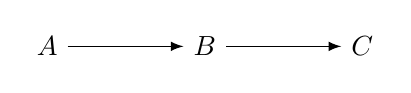
\begin{tikzpicture}[-latex,auto ,node distance =1 cm and 2cm ,on grid ,
    semithick ,
    variable/.style ={ circle ,top color =white , 
    draw , text=blue , minimum width =1 cm},
    kernel/.style={rectangle,draw}
    ]

\node (A) {$A$};
\node (B) [right = of A] {$B$};
\node (C) [right = of B] {$C$};
\draw (A) -- (B);
\draw (B) -- (C);
\end{tikzpicture}
\end{center}

Can be completed either by $\overline{\mathcal{G}}_1$ or $\overline{\mathcal{G}}_2$:
\begin{center}
    \begin{tikzpicture}[-latex,auto ,node distance =1 cm and 2cm ,on grid ,
    semithick ,
    variable/.style ={ circle ,top color =white , 
    draw , text=blue , minimum width =1 cm},
    kernel/.style={rectangle,draw}
    ]

\node (A1) {$A$};
\node (B1) [right = of A1] {$B$};
\node (C1) [right = of B1] {$C$};
\node (G1) [below right = of A] {$\overline{\mathcal{G}}_1$};
\draw (A1) -- (B1);
\draw (B1) to (C1);
\draw (A1) to [bend left] (C1);
\node (A2) [right = of C1] {$A$};
\node (B2) [right = of A2] {$B$};
\node (C2) [right = of B2] {$C$};
\node (G2) [below right = of A] {$\overline{\mathcal{G}}_2$};
\draw (A2) -- (B2);
\draw (B2) to (C2);
\draw (C2) to [bend right] (A2);
\end{tikzpicture}
\end{center}

\end{definition}

\begin{theorem}[Subgraph compatibility for causal invariance networks]\label{th:subgraph_compatibility}
Given some distribution $\mu\in \Delta(\mathcal{F})$ that is compatible with some subgraph $\mathcal{G}'$ of $\mathcal{G}_M$, a causal invariance network will automatically have the property that every distribution $\nu$ in the range of $\mathscr{T}^{I}_{\mathcal{G}_M}(\mu)$ will be compatible with $\mathcal{G}'$ (see definition \ref{def:causal_prospect} for the definition of the range of $\mathscr{T}^{I}_{\mathcal{G}_M}(\mu)$).
\end{theorem}

\begin{proof}
By assumption, for each $\RV{W}_i\in \RV{W}$,
\begin{align}
    P_\mu(\RV{W}_i|\PA{\mathcal{G}_M}{\RV{W}_i}) = P_\mu(\RV{W}_i|\PA{\mathcal{G}'}{\RV{W}_i}) \label{eq:independence}
\end{align}

Consider any $\nu_S\in \text{Range}\mathscr{T}^{I}_{\mathcal{G}_M}(\mu)(\cdot|e_S)$ where $S\subset\{0,..,N\}$ and $e_S\in E_S\subset D$ defined as above.

Suppose $e_S=f(w,S)$ and take any $S'\subset\{0,..,N\}$. By condition 1 we have for any $i\in S$
\begin{align}
    P_{\nu_S}(\RV{W}_i|\RV{W}_{S'}) = \llbracket \RV{W}_i = p_{\{i\}}(w) \rrbracket \label{eq:hard_int}
\end{align}

And by condition 2, for any $i\not\in S$ we have
\begin{align}
    P_{\nu_S}(\RV{W}_i|\PA{\mathcal{G}_M}{\RV{W}_i}) =P_\mu(\RV{W}_i|\PA{\mathcal{G}_M}{\RV{W}_i}) \label{eq:invariance}
\end{align}

Because $\mathcal{G}_M$ is fully connected, by the product rule we can always write
\begin{align}
    P_{\nu_S}(\RV{W}) &= \prod_{i\in \{0,..,N\}} P_{\nu_S}(\RV{W}_i|\PA{\mathcal{G}_M}{\RV{W}_i})\\
                      &= \prod_{i\in S}\llbracket \RV{W}_i = p_{\{i\}}(w) \rrbracket \prod_{j\in S^C}P_{\nu_S}(\RV{W}_j|\PA{\mathcal{G}_M}{\RV{W}_j})\\
                      &= \prod_{i\in S}\llbracket \RV{W}_i = p_{\{i\}}(w) \rrbracket \prod_{j\in S^C}P_{\mu}(\RV{W}_j|\PA{\mathcal{G}'}{\RV{W}_j})\label{eq:subformu}\\
                      &= \prod_{i\in S}P_{\nu_S}(\RV{W}_j|\PA{\mathcal{G}'}{\RV{W}_j}) \prod_{j\in S^C}P_{\mu}(\RV{W}_j|\PA{\mathcal{G}'}{\RV{W}_j}) \label{eq:clearly_markov}
\end{align}

Where line \ref{eq:subformu} follows from Eq. \ref{eq:independence} and \ref{eq:invariance} and line \ref{eq:clearly_markov} follows from Eq. \ref{eq:hard_int}. $P_{\nu_S}(\RV{W})$ is clearly compatible with $\mathcal{G}'$.
\end{proof}

Theorem \ref{th:subgraph_compatibility} suggests a connection between causal Bayesian networks and causal invariance networks. In particular, a causal Bayesian network $\mathscr{T}^B_\mathcal{G}$ is related to any causal invariance network $\mathscr{T}^I_{\overline{\mathcal{G}}}$ where $\overline{\mathcal{G}}$ is some completion of $\mathcal{G}$. In particular, for any $\mu$ such that $\mathscr{T}^B_\mathcal{G}(\mu)\neq \emptyset$, $\mathscr{T}^B_\mathcal{G}(\mu)=\mathscr{T}^I_{\overline{\mathcal{G}}}(\mu)$.

It's not completely clear what is to be gained by this correspondence, but it seems like separating interventional invariance and conditional independence assumptions might be helpful.

\subsubsection{Complexity Measures}

Given some joint probability distribution $P(\RV{V})=P(\RV{V}_0,..,\RV{V}_n)$, suppose we have some permutation-dependent ``divergence'' $C$. That is, given some ``divergence'' $D$
\begin{align}
    C(P(\RV{V})\|Q(\RV{V});s_\alpha) &= \sum_{\alpha_i\in s_\alpha} D(P(\RV{V}_{\alpha_i}|\RV{V}_{\alpha_{<i}})\|Q(\RV{V}_{\alpha_i}|\RV{V}_{\alpha_{<i}}))
\end{align}

$D$ is a divergence in the sense that it is positive semidefinite and $D(F\|G)=0$ iff $F=G$. It is a ``divergence'' in that $F$ and $G$ are Markov kernels rather than probability distributions.

Suppose we have a probability space $(\Omega,\mathcal{F},\mu)$, a decision space $(D,\mathcal{D})$, a causal prospect $\mathscr{T}$ and random variables $\RV{V}=\{\RV{V}_0,..,\RV{V}_n\}$. If for some $d\in D$ our causal prospect demands that $P_{\nu K(\cdot;d)}(\RV{V}_i)=\delta_x(\RV{V}_i)$ for all $\nu\in \Delta(\mathcal{F})$ and $K\in \mathscr{T}(\nu)$ then $C(P_\mu(\RV{V})\|P_{\nu K(\cdot;d)}(\RV{V});s_\alpha)$ is not minimised if
\begin{align}
    P_{\nu K(\cdot;d)}(\RV{V}) = \delta_x(\RV{V}_i)\prod_{\alpha_i\in s_\alpha\setminus\{i\}} P(\RV{V}_{\alpha_i}|\RV{V}_{\alpha_{<i}})
\end{align}

I made a mistake, I thought it would be minimised. A good question, though, is: when would it be minimised?

It has been suggested that we use Kolmogorov complexity to determine the ``correct'' factorisation\cite{lemeire_replacing_2013}. In particular, take the set $S_n$ of permutations of $n$ elements, and for some $s_i\in S$ we have $s_\alpha = \{\alpha_0,..,\alpha_n\}$. Suppose that the ``correct'' factorisation by $s_\alpha \in S_n$:
\begin{align}
    P(\RV{V})=\prod_{\alpha_i\in s_\alpha} P(\RV{V}_{\alpha_i}|\RV{V}_{\alpha_{<i}})
\end{align}
Then, letting $K(x)$ be the Kolmogorov complexity of $x$, it is suggested that, very roughly speaking, for $s_\beta \neq s_\alpha$
\begin{align}
    K(P(\RV{V})) &\approx \sum_{\alpha_i\in s_\alpha} K(P(\RV{V}_{\alpha_i}|\RV{V}_{\alpha_{<i}})) \label{eq:complexity_equality}\\
    K(P(\RV{V})) &< \sum_{\beta_i\in s_\beta}K(P(\RV{V}_{\beta_i}|\RV{V}_{\beta_{<i}}))\label{eq:complexity_inequality}
\end{align}

That is, there is some canonical permutation of variables $s_\alpha \in S_n$ such that the Kolmogorov complexity of the sum of the terms in the factorization is minimized.


\bibliographystyle{plain}
\bibliography{references.bib}


\end{document}
